\item \textbf{{[}DHS/PRELIM/9597/2019/P1/Q3{]} }

From 2021 onwards, the Primary School Leaving Exam (PSLE) will be
scored with wider bands, replacing the current T-scores. 

Each subject will be scored using 8 bands known as Achievement Levels
(AL), with AL 1 being the best score and AL 8 being the lowest score.
The student\textquoteright s PSLE Score will be the sum of the four
subject scores. The PSLE Score will range from 4 (best) to 32. 
\begin{center}
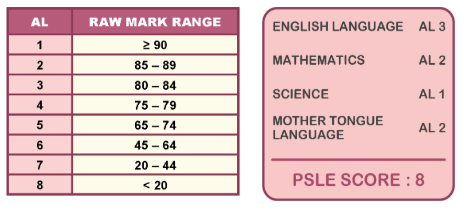
\includegraphics[width=0.5\paperwidth]{C:/Users/Admin/Desktop/Github/question_bank/LyX/static/img/9597-DHS-2019-P1-Q3}
\par\end{center}

Secondary 1 posting will continue to be based on academic merit, using
the PSLE Score. 

Each student will submit a list of 6 schools in order of preference.
If two students with the same score are being considered for the last
place in a school, the following tie-breakers will be used: 
\begin{itemize}
\item Citizenship - priority given to Singapore Citizens (SC), then Singapore
Permanent Residents (PR), then International Students (IS) 
\item Choice order of schools - priority given to the student who indicates
a certain school as a higher choice 
\item Computerised balloting 
\end{itemize}
The file \texttt{PSLE21.txt} contains the application information
of 400 Primary 6 students of a primary school with the following structure:

\texttt{<StudentID>,<EnglishLanguageMark>,<MathematicsMark>,<ScienceMark>,<MotherTongueLangueMark>,<Citizenship>,<SchoolChoice1>,<SchoolChoice2>
,<SchoolChoice3> }

You may assume that in this school all students study subjects at
the standard level. Also, all of them have made up their mind to only
apply to 3 schools of their choice. If a student is unable to get
admission to a school of their choice, they will be posted to SchoolD.

It is decided to process and store the following application information
about the student in 4 linked lists. Each linked list pertain to the
vacancy positions of the 4 schools. Schools A, B and C have 120, 150
and 80 available places. The data to be stored in each linked list
node include: PSLE score, student ID, citizenship and the 3 school
choices. 

\subsection*{Task 3.1 }

Write program code to read in and store the contents of the file \texttt{PSLE21.txt}
in a dictionary \texttt{students} with key \texttt{StudentID} and
value the computed PSLE score, citizenship and three school choices.
Display the first 10 dictionary entries in \texttt{students}. 

\subsection*{Evidence 11}

Program code. \hfill{}{[}6{]}

\subsection*{Evidence 12 }

Screenshot for first 10 dictionary entries in \texttt{students}.\hfill{}
{[}1{]}

\subsection*{Task 3.2 }

Using OOP where appropriate, write program code to declare and initialise
the necessary classes. Insert the 400 students from the \texttt{students}
dictionary in Task 3.1 to the appropriate linked lists in your main
program driver code. 

\subsection*{Evidence 13 }

Program code. \hfill{}{[}16{]}

\subsection*{Evidence 14 }

Screenshots for the first 5 entries in each linked list. \hfill{}{[}4{]}

\subsection*{Task 3.3 }

Students \texttt{P351} and \texttt{P365} who were previously Singapore
Permanent Residents (PR) have successfully become Singapore Citizens
(SC). Write the necessary program code to update their citizenship
status and new secondary 1 posting order. 

\subsection*{Evidence 15}

Program code. \hfill{}{[}5{]}

\subsection*{Evidence 16 }

Screenshots. \hfill{}{[}2{]}

\subsection*{Task 3.4}

Student \texttt{P286} has decided to emigrate to another country with
his/her parents. Write the necessary program code to remove him/her
from his/her existing allocation and perform the necessary adjustments
to fill up the vacancy. 

\subsection*{Evidence 17}

Program code. \hfill{}{[}5{]}

\subsection*{Evidence 18 }

Screenshot.\hfill{} {[}1{]}